\chapter{Results and Discussion} \label{chp:4}

The methods of this investigation, as described in chapter \ref{chp:3}, lead to the generation of a directed graph, generated from the log file, indicating the flow of model information as can be seen in figure \ref{Graph_modDistro}. 

\begin{figure}[p] \label{Graph_modDistro}
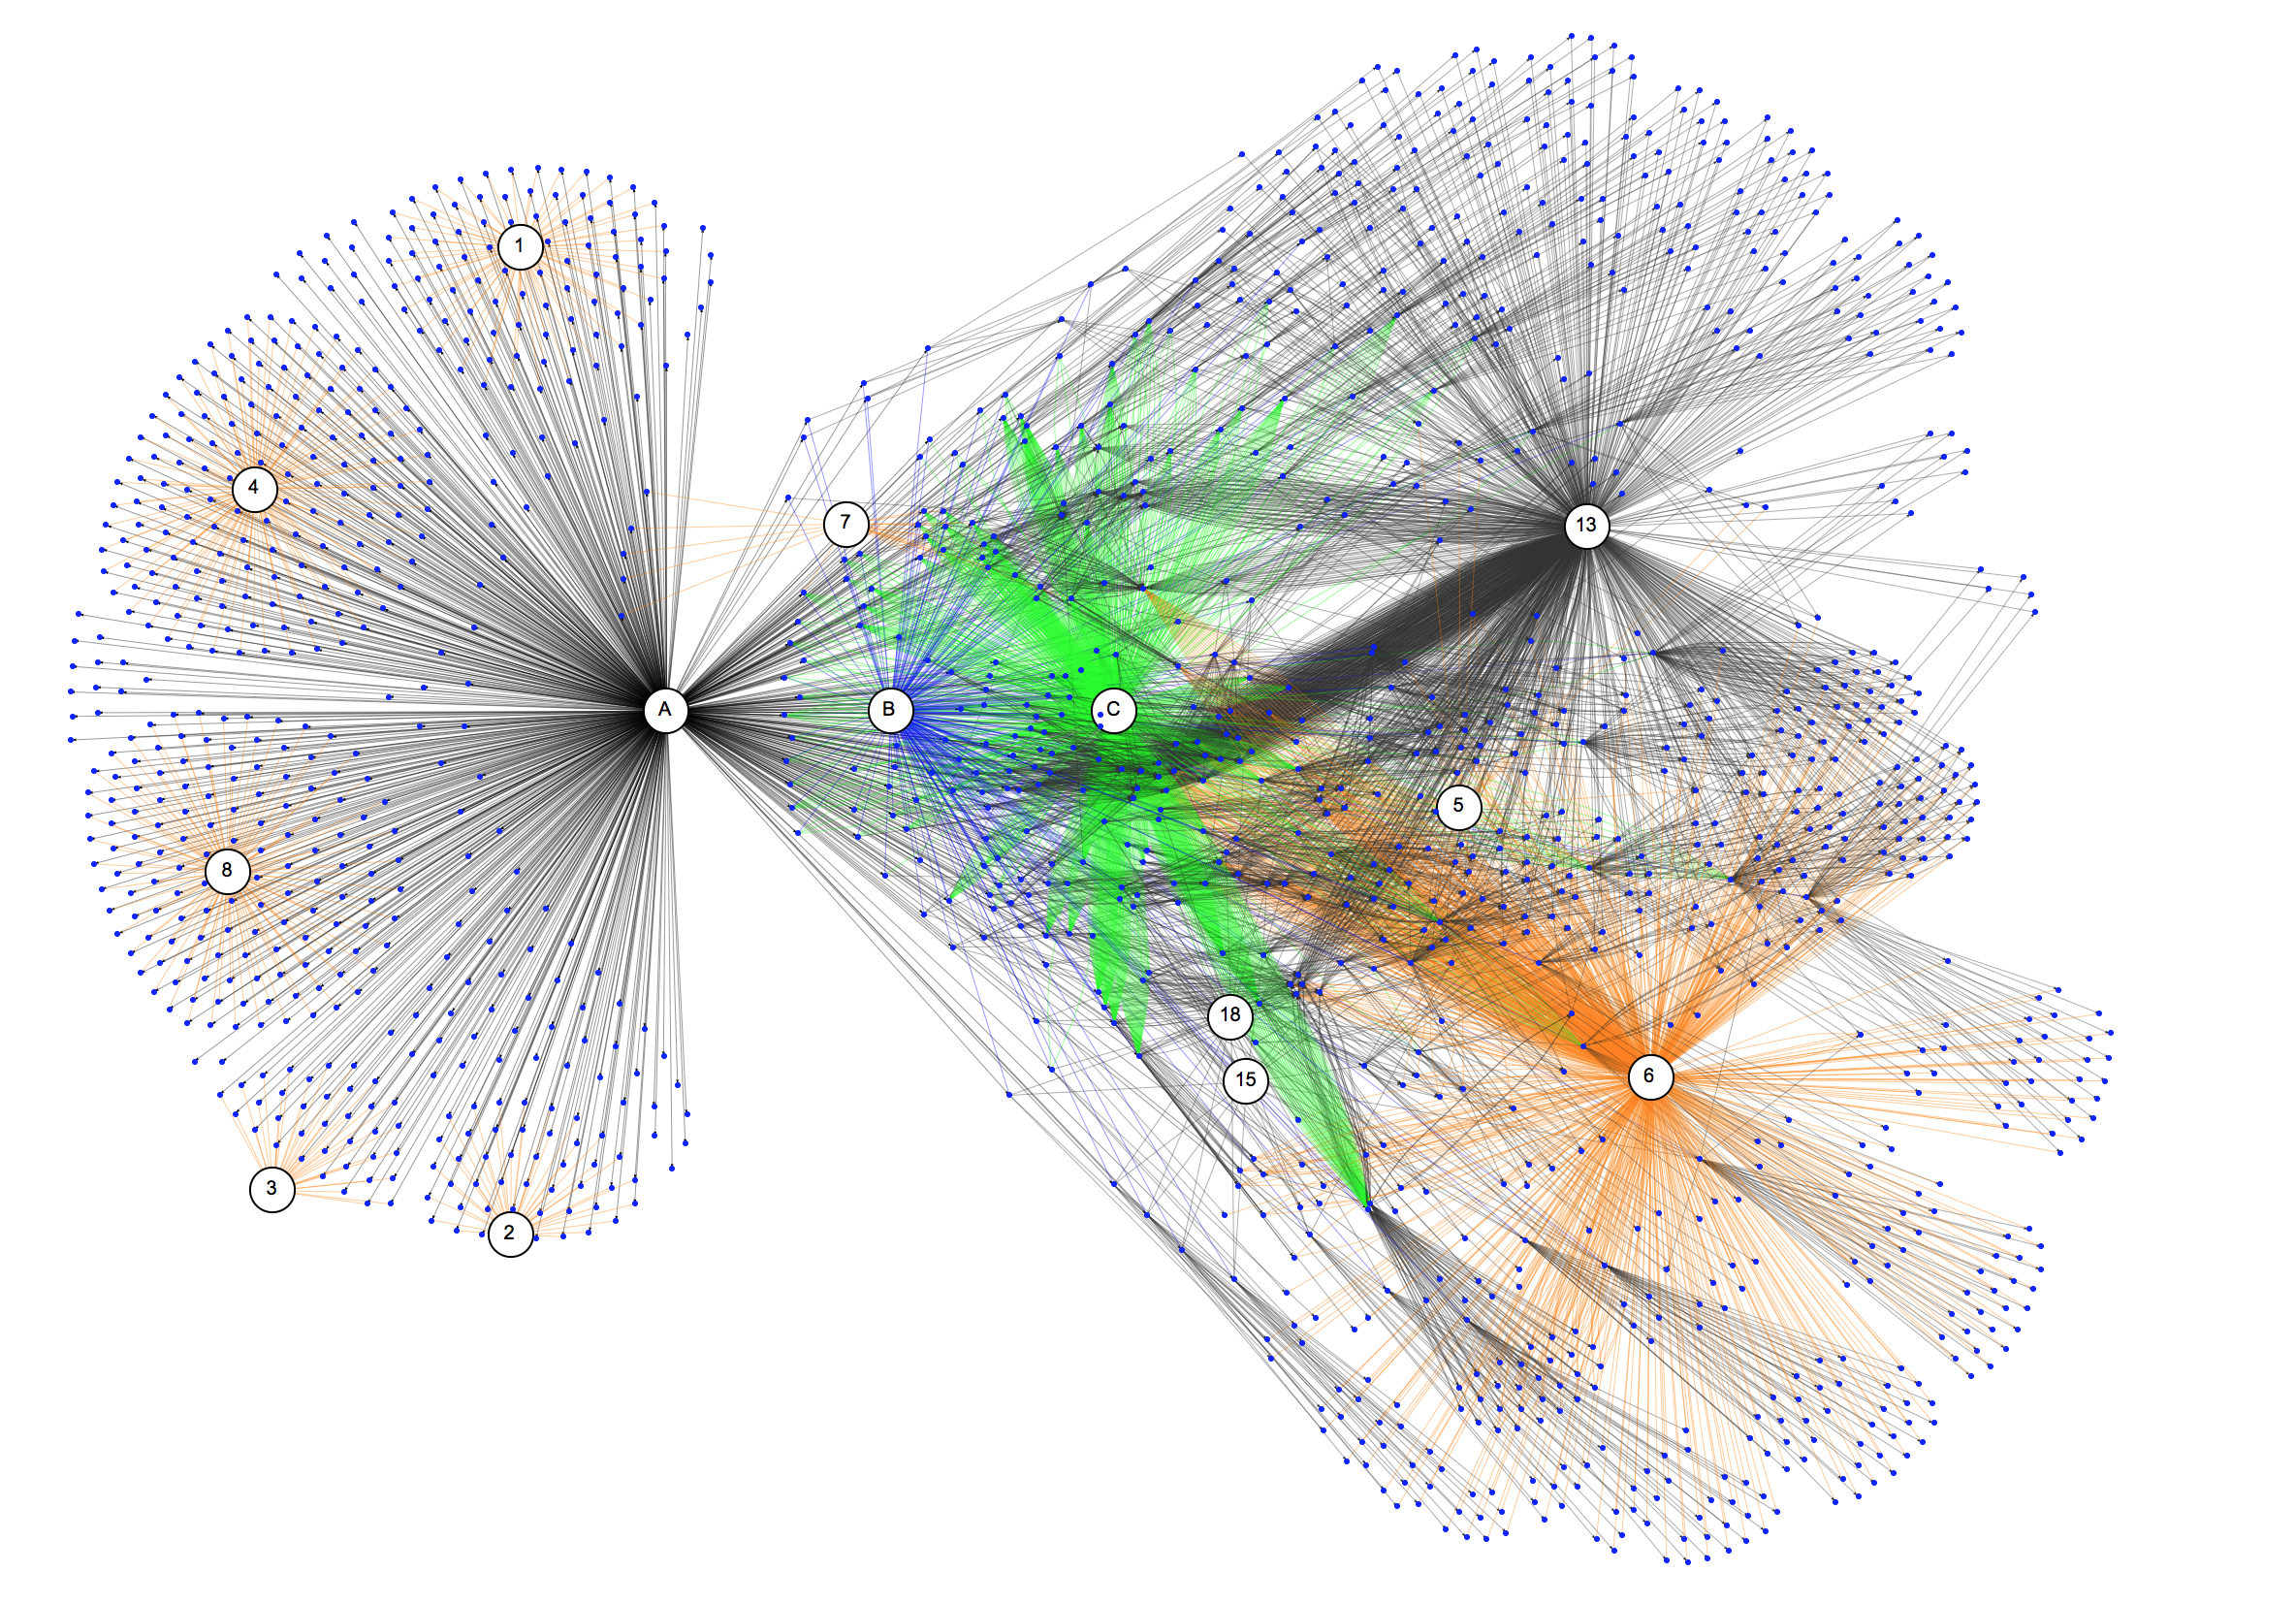
\includegraphics[width=1\textwidth]{figs/Digraph.png}
\centering
\caption{Directed graph indicating the flow of models as they are filtered by the algorithm described in chapter \ref{chp:3}. 
Important checkpoints are indicated by letters, with $A \rightarrow{}$ All models, $B \rightarrow{}$ Has reversible rates and $C \rightarrow{}$ Initial check functions passed. Filter criteria is labeled by number, with $1 \rightarrow{}$ No stoichiometries, $2 \rightarrow{}$ Events, $3 \rightarrow{}$ Piece-wise, $4 \rightarrow{}$ Oscillatory, $5 \rightarrow{}$ Division by zero, $6 \rightarrow{}$ Flux summation error, $7 \rightarrow{}$ Timed out, $8 \rightarrow{}$ No reversible reactions, $9 \rightarrow{}$ Import error, $10 \rightarrow{}$ Negative FCC, $11 \rightarrow{}$ Steady-state error, $12 \rightarrow{}$ Division by zero, $13 \rightarrow{}$ No product or substrate, $14 \rightarrow{}$ Replacement errors, $15 \rightarrow{}$ Small maximum elasticity coefficient, $16 \rightarrow{}$ No reversible reactions, $17 \rightarrow{}$ Flux calculation error and $18 \rightarrow{}$ No flux results generated.}
\end{figure}

This figure allows one to gain an overview of the model space. The models of importance were ones leading towards $c$ with green line, it is however clear that many models did not meet the requirements, $86\%$ to be exact. The final data contains reactions from 111 models, yielding 843 data points on disequilibrium ratio and flux control co\"efficient. The probability distributions of this data can be seen in figure \ref{TwoResPDF}.

A probability density function of the distribution, normalized via Gaussian kernel, was visualized by a contour plot. This plot can be seen at two resolutions in figure \ref{TwoResPDF}. It is clear that there exists a tendency for reactions close to equilibrium to not have a large degree of own flux control. As can be seen from figure \ref{TwoResPDF} $a$, there is no representative reaction with a control co\"eficient larger than $0.4$. On the opposite side of the scale it is observed that reactions with a larger than $0.4$ control co\"efficient reside within the region of $\rho < 0.1$. At a higher resolution however, figure \ref{TwoResPDF} $b$ indicates that reactions close to equilibrium ($\rho > 0.9$), with larger than $0.4$ flux control co\"efficients  do exist, albeit few. The \rho separation values chosen above, can be seen in figure \ref{PredictionConfidence}. These values echo the conclusion by \citeauthor{Rohwer2009} as discussed in chapter \ref{chp:2}.

To gain some degree of confidence in the visual findings, the data was utilized in the training of three separate neural networks. The probability density functions of the predicted flux control co\"efficients were visualised on the same axes as can be seen in figure \ref{PredConf}

\begin{figure}[p] \label{TwoResPDF}
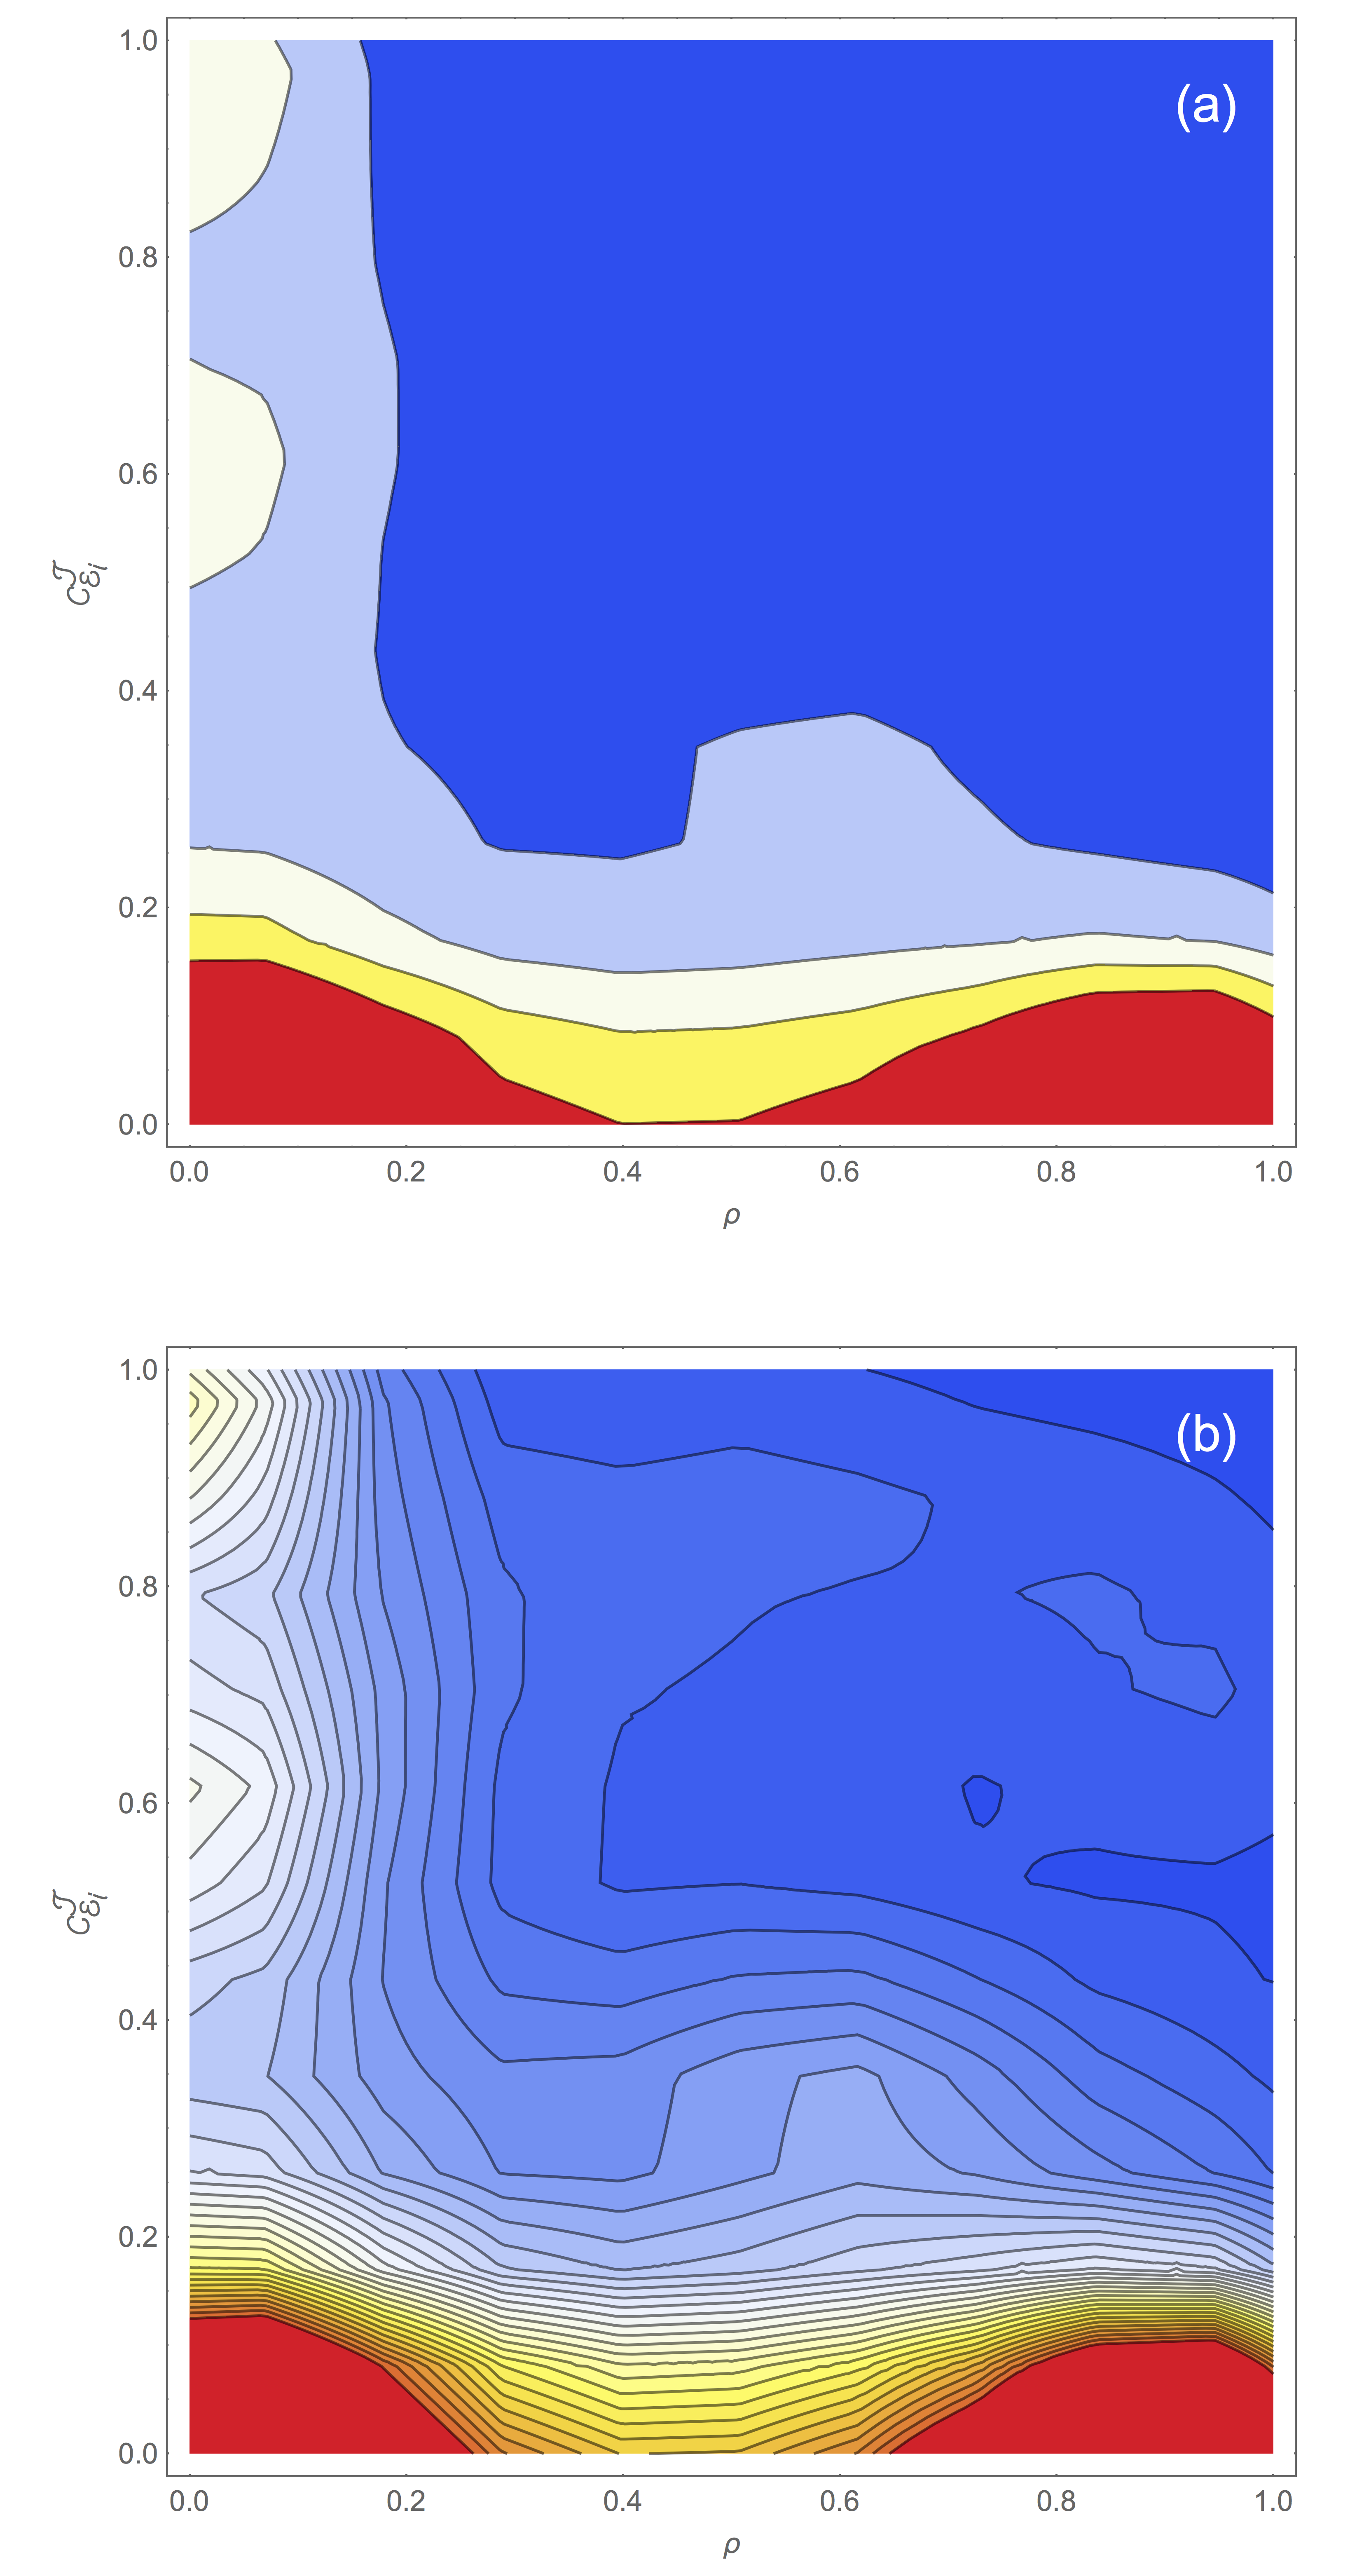
\includegraphics[width=0.8\textwidth]{figs/TwoResPDF.png}
\centering
\caption{Two resolutions was obtained by varying the contour amount visualized, $a = 4$ and $b = 30$, from the probability density function calculated in chapter \ref{chp:3}. This data is on the disequilibrium ratio ($\rho$) and the own flux control coefficient ($C_{E_i}^J$), normalized to the probability space of one. Red and blue respectively denote high and low density areas of data points.}
\end{figure}

\begin{figure}[p] 
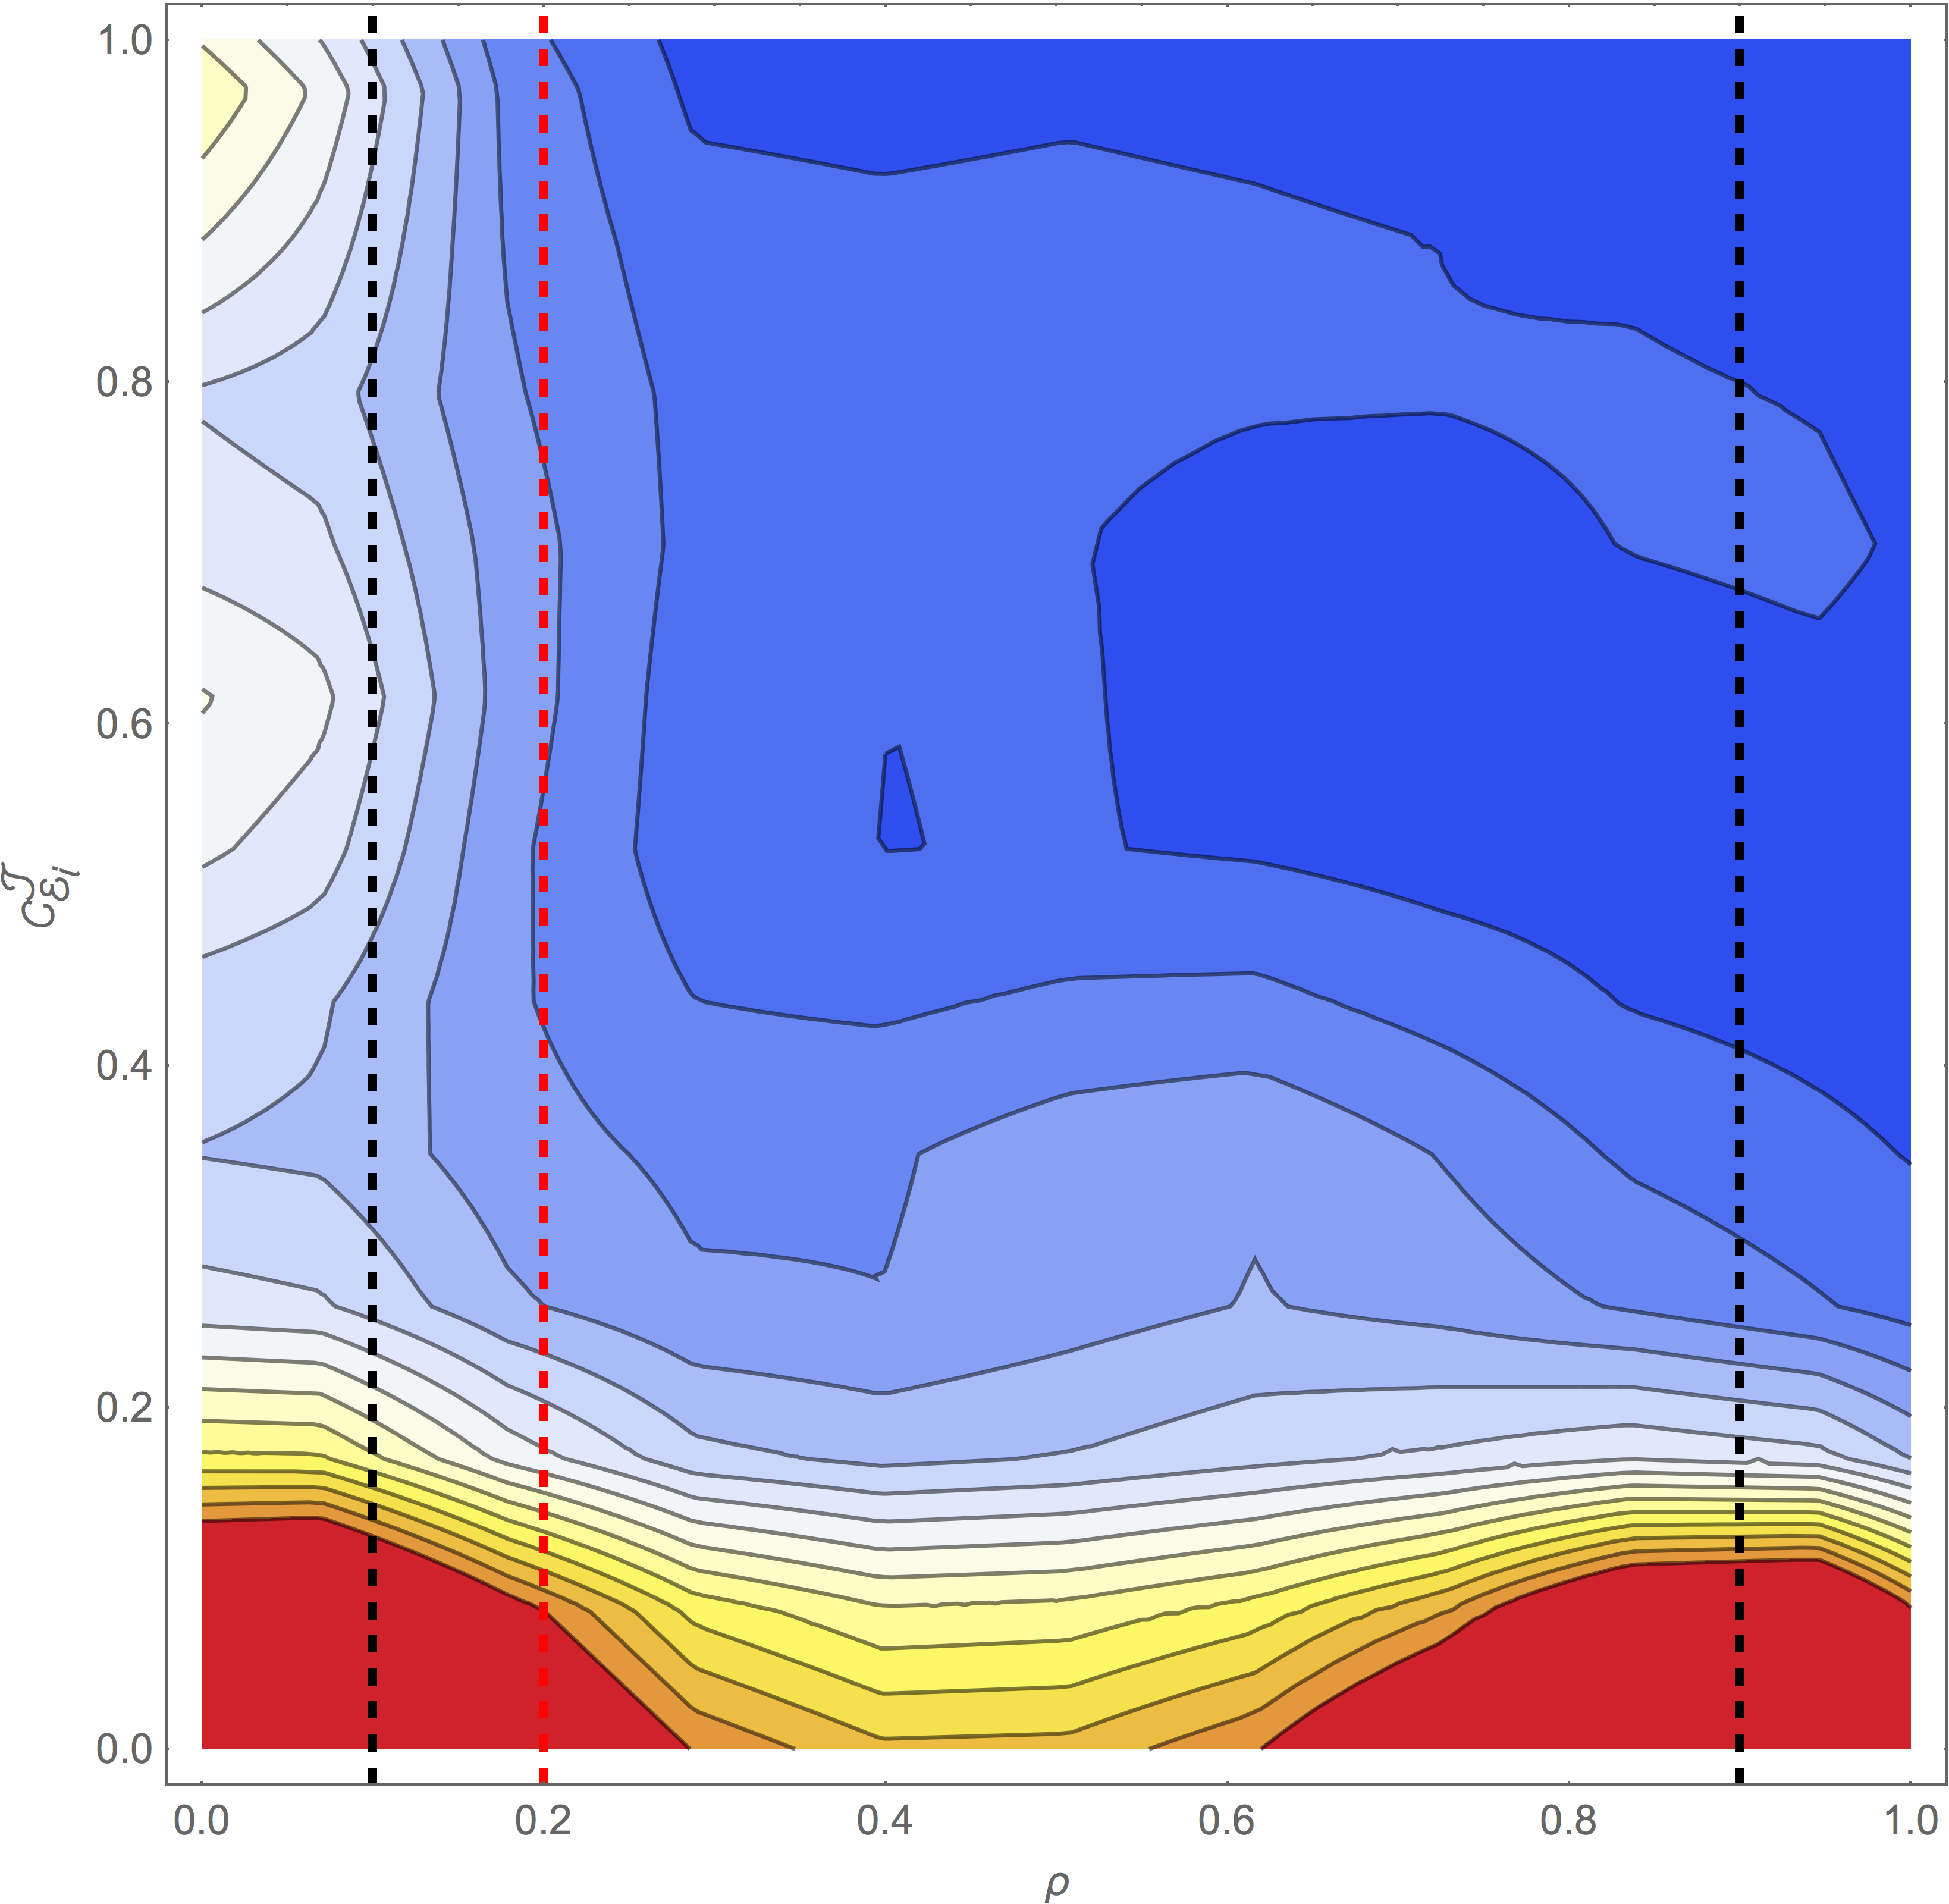
\includegraphics[width=0.8\textwidth]{figs/LitCompare.png} \label{LitCompare}
\centering
\caption{Probability density function of data gathered. This data is on the disequilibrium ratio ($\rho$) and the own flux control coefficient ($C_{E_i}^J$), normalized to the probability space of 1. Red and blue respectively denote high and low density areas of data points. The black (\citeauthor{Rohwer2009}) and red (\citeauthor{ROLLESTON1972}) dashed lines indicate respective authors views, as referred to in chapter \ref{chp:2}, on probable conditions of dominating contributions to regulation.}

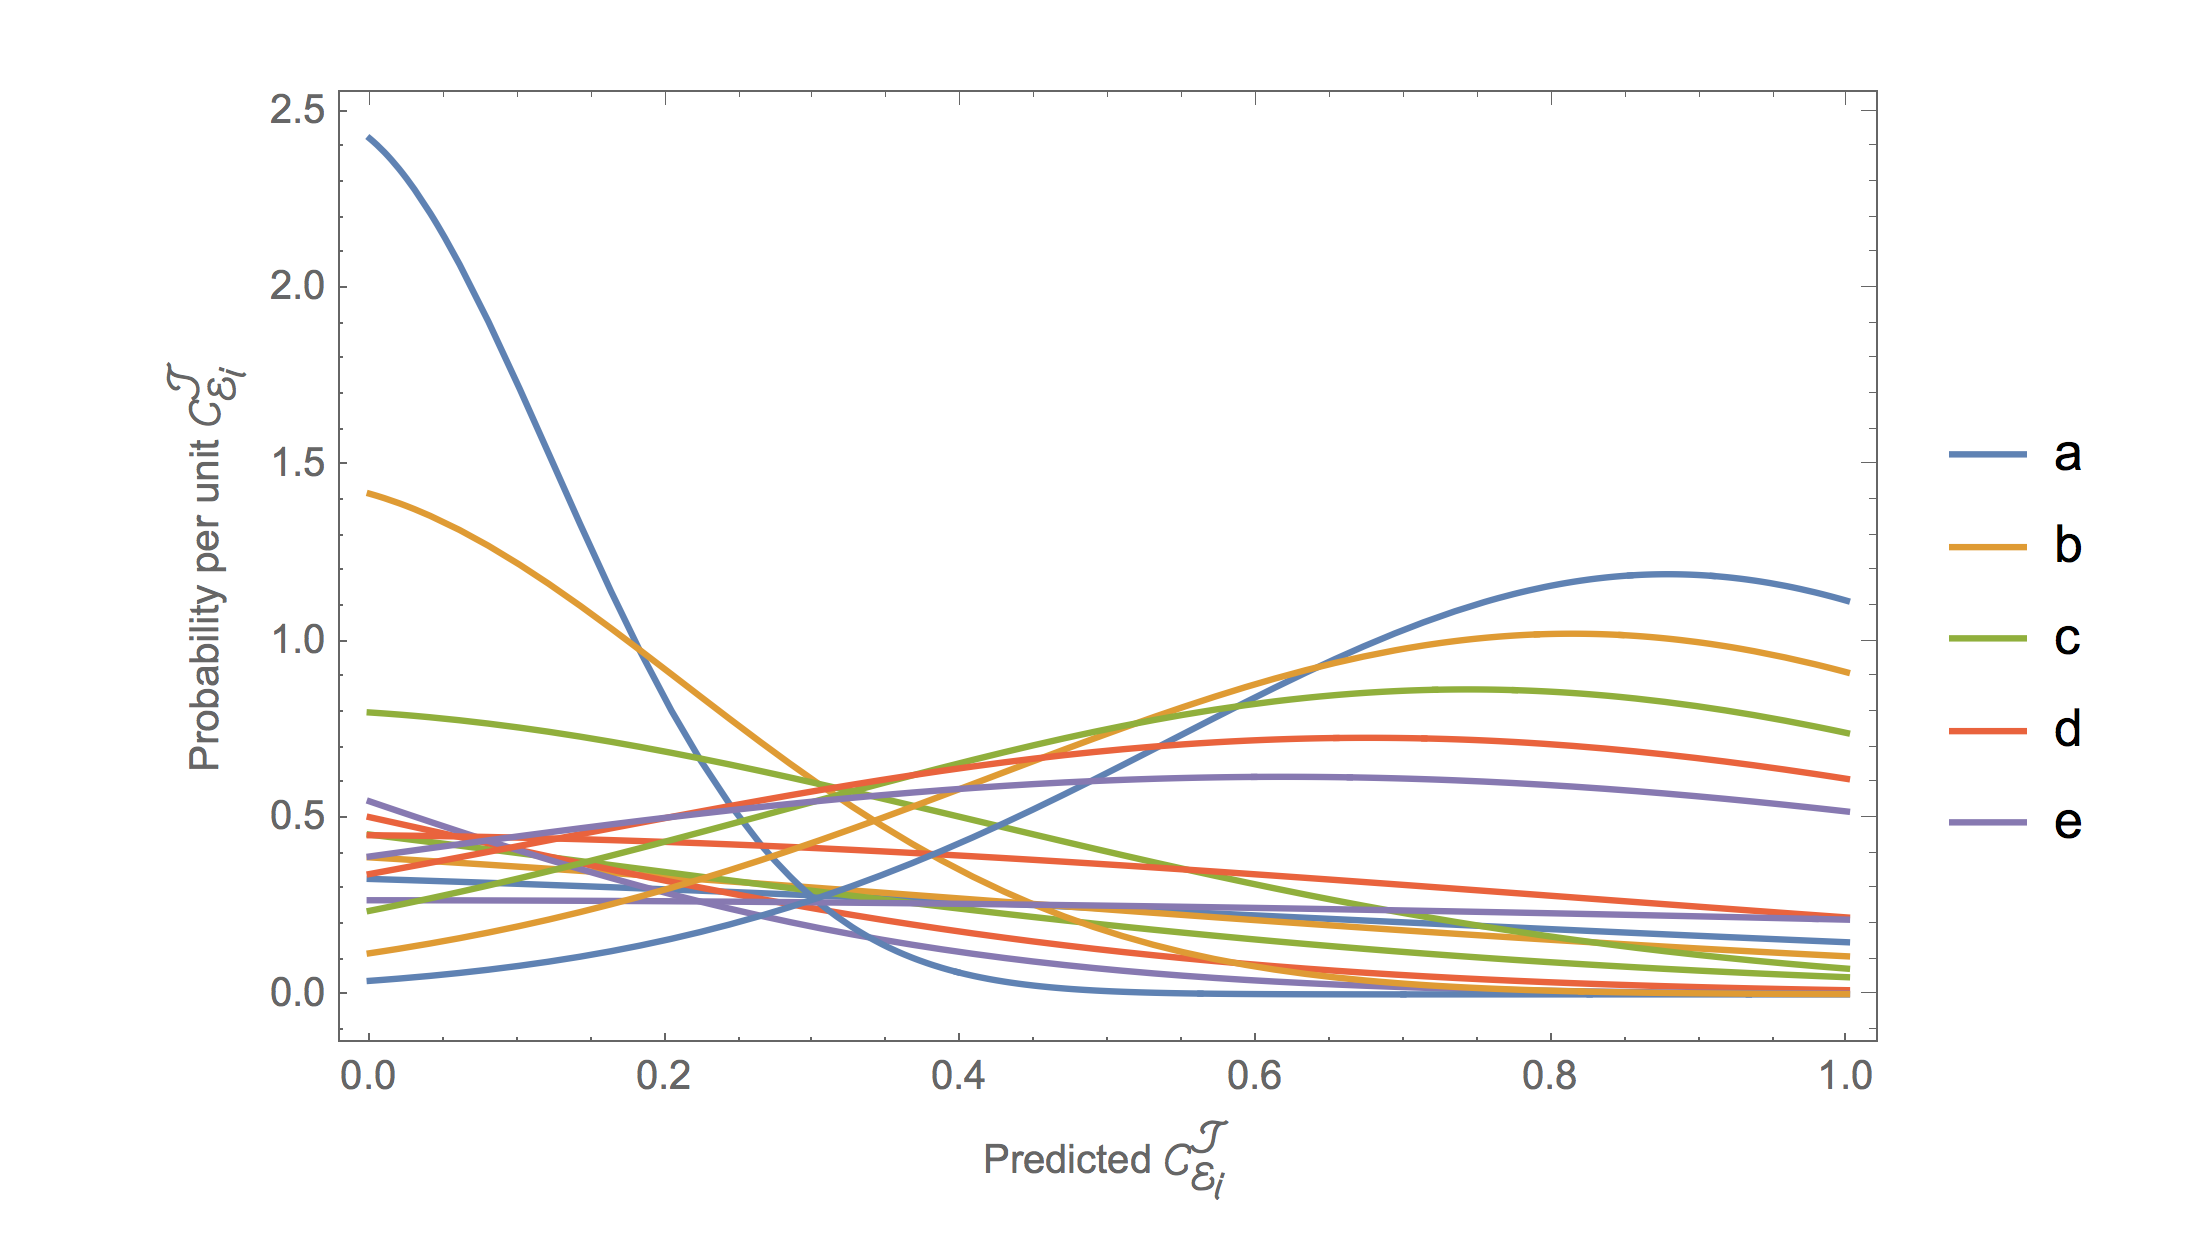
\includegraphics[width=1\textwidth]{figs/PredConf.png} \label{PredictionConfidence}
\centering
\caption{Probability density functions of estimates on flux control co\"efficients. Predictions were made at six disequilibrium ratio values, from three respective Mathematica neural network predictor functions, as referred to in \ref{chp:3}. The chosen disequilibrium ratios were $a = 0.01$, $b = 0.25$, $c = 0.50$, $d = 0.75$, and $e = 0.99$ respectively.}
\end{figure}


Four hypothesis were set in order to further evaluate the gathered data. Based on the premise of covering all possible combinations of variables the first of these postulates that; large flux control co\"efficients are witnessed at small disequilibrium ratios.

\begin{equation}
    \rho \ll 1 \Longrightarrow C_{E_i}^J \gg 0
\end{equation}

The second is derived from the reciprocal supposition, where large flux control co\"efficients necessarily relates to small disequilibrium ratios.

\begin{equation}
    C_{E_i}^J \gg 0 \Longrightarrow \rho \ll 1
\end{equation}

With the first two hypothesis relating distances far from equilibrium to control, the third and forth relates to the opposite. With disequilibrium ratios approaching unity, the third hypothesis necessitates a small observed flux control co\"efficient.

\begin{equation}
    \rho \approx 1 \Longrightarrow C_{E_i}^J \ll 1
\end{equation}

While the final hypothesis views disequilibrium ratios as necessarily approaching unity where small flux control co\"efficients are concerned.

\begin{equation}
    C_{E_i}^J \ll 1 \Longrightarrow \rho \approx 1
\end{equation}

Applying these four hypothesis to the probability density function obtained from the data, one can gain insights into how thermodynamic states influence control behaviour. 


